\subsection*{Sensor theory}
Sensor fusion can be observed everywhere e.g., living animals uses all of its senses to survive daily, an animal cannot hunt using its eyes only, it has to combine its sense of smell, eyes and hearing to hunt the pray\cite{animal}. Sensor fusion theory is not only found in the living species it is found in cars, planes, computers and so on ans this to enhance performance \cite{animal}. In this project sensor fusion will be used to enhance the accuracy of the dinghy's position and velocity. The fusion will be between a GPS and the IMU.\\ 
The GPS's accuracy is not uniform since it might be buildings reflections, atmospherics delays or clock bias errors \cite{boken}. Using only information provided by a IMU is not sufficient either since the sensors will drift after time, using the sensors only for short time will give accurate readings.  


\subsection{Kalman Filter}
A popular filter to use when doing sensor fusion is to use a Kalman filter, (KF). The Kalman Filter is a recursive filtering method for discrete data, the algorithm was developed by an Hungarian mathematician Rudolf (Rudi) Emil Kalman in 1960 \cite{boken}. Its popular to use due to its efficiency when calculating predictions. \cite{kf eff}


Since everything is nonlinear in the universe, many systems cannot be modeled as linear \cite{nonlinear} and therefore Extended Kalman, (EKF) Filter has to be applied when this cases arises. The EKF linearizes the system around its working points. When deriving the dynamics of the system the decision can be made which type of filter will be used. The model is given as a linear equation

\begin{align}
&\textrm{State equation} \qquad x_k=F_{k-1}x_{k-1}+v_{k-1}\\
& \textrm{Observation equation} \qquad z_k=H(x_k)+w_k
\end{align}
where $v_k$ and $w_k$ is the process noise and measurement noise, respectively both assumed to be zero mean Gaussian noise with covariance matrices $Q_k$ and $R_k$, i.e. $v_k\in\mathcal{N}(0, Q_{k-1})$ and $w_k\in\mathcal{N}(0, R_k)$.

\begin{align}
&\textrm{Predict state estimate:} \qquad \hat{x}_{k|k-1}=F_k\hat{x}_{k|k-1}+Gv_{k-1}\\
&\textrm{Predict covariance matrix:}\qquad P_{k|k-1}=F_{k}P_{k-1|k-1}F^T_{k}+Q_{k}\\
\label{eq.measurement}
&\textrm{measurement residual}\qquad \tilde{y}_k=z_k-H_k\hat{x}_{k|k-1}\\
&\textrm{Innovation covariance}\qquad S_k=H_kP_{k|k-1}H_k^T+R_k \\
&\textrm{Optimal Kalman gain}\qquad K_k=P_{k|k-1}H_k^TS_k^{-1}\\
\label{eq.Update}
&\textrm{Update state estimate}\qquad \hat{x}_{k|k}=\hat{x}_{k|k-1}+K_k\tilde{y}_k\\
&\textrm{Update covariance estimate}\qquad P_{k|k}=(I-K_kH_k)P_{k|k-1}\\
&\textrm{Measurement post-fit residual} \qquad \tilde{y}_{k|k}=z_k-H_k\hat{x}_{k|k}
\end{align}
If Eq.\eqref{eq.measurement} and Eq.\eqref{eq.Update} is analyzed we see that depending on how much we believe in the observations that are observed will affect the gain matrix. Consider Fig. \ref{kalman_algo} as a map of how the algorithm works and Fig. \ref{kalman_system} as a description on how the system works.
\begin{figure}[H]
\centering
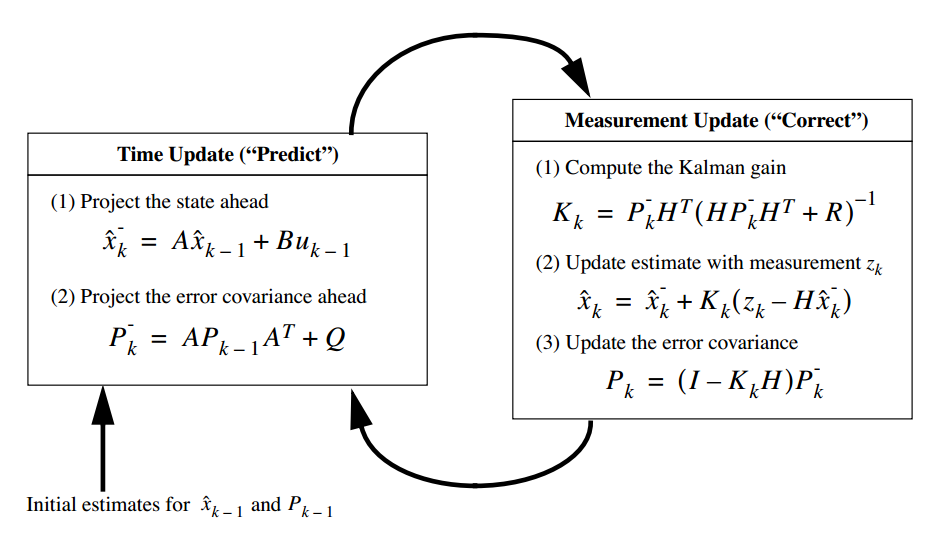
\includegraphics[width=0.8\textwidth]{Figures/kalman_algo.png}
\caption{Kalman Filter prediction algorithm}
\label{kalman_algo}
\end{figure}

\begin{figure}[H]
\centering
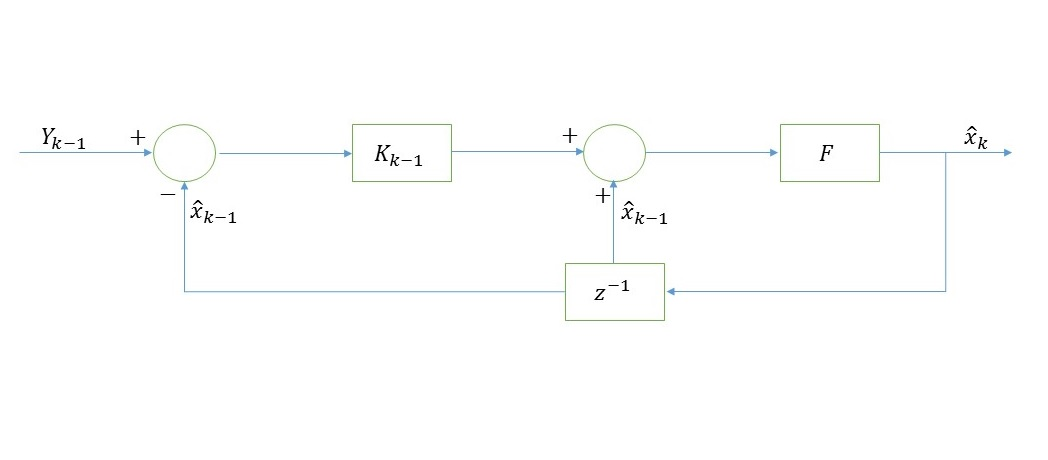
\includegraphics[width=0.8\textwidth]{Figures/Bild1.JPG}
\caption{System diagram of Kalman prediction}
\label{kalman_system}
\end{figure}

\subsection*{Integration GPS/INS}
It exist different types of integration levels most common are loosely, tightly and ultra-tightly coupled. The two last types are used when the output from the GPS receiver is its pseudo-range and carrier-range. Since the GPS receiver that is used in this project uses NMEA standard, the output from the GPS will be the calculated position, velocity and heading. Then using a loosely coupled integration is preferred, profits using loose coupled are that its easiest way of fusion sensors together. Consider Fig. as how the system works between the different sensors.

\begin{figure}[H]
\centering
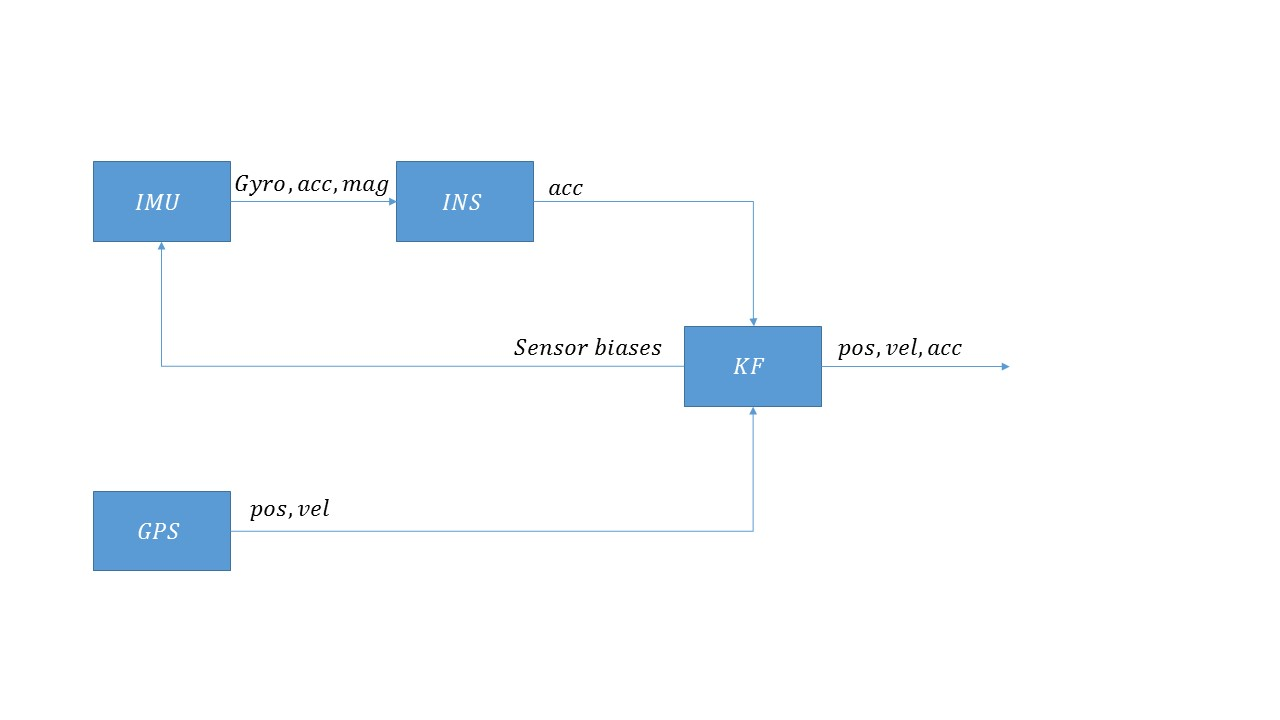
\includegraphics[width=0.8\textwidth]{Figures/loose_coup.JPG}
\caption{GPS/INS with loose integration}
\label{kalman_system}
\end{figure}

\subsection*{Kalman Filter Model}
The states that we want to observe are.
\begin{align}
\bar{x}=&
\begin{bmatrix}
x^{pos}\quad[m]\\
y^{pos}\quad[m]\\
v^{x}\quad[m/s]\\
v^{y}\quad[m/s]\\
\end{bmatrix}
\end{align}
$x_{pos}$ and $y_{pos}$ is the position in x and y direction, respectively, velocity, $v$, acceleration, $a$. The coordinate system that is used for calculations are the \emph{WGS-84}. See Fig. \ref{bat} for a geometrical perspective.

The Kalman filter calculates estimates of the true values of states recursively over time using incoming measurements and a mathematical process model, i.e. it uses $x_{k-1}$ to calculate $x_k$. Hence a mathematical model has to be derived describing the process, the GPS will provide heading position and velocity, the IMU will provide acceleration in $xy$-direction.\\
The model will not make an assumption that the acceleration is constant under the sampling times, this since the sampling period is $1Hz$. The process model is derived using kinematics using only $xy$-directions.
	
\begin{align}
x^{pos}_{k}&=x^{pos}_{k-1}+\Delta tv^{x}_{k-1}+\frac{1}{2}\Delta t^2a^x_{k-1}\\
y^{pos}_{k}&=y^{pos}_{k-1}+\Delta tv^{y}_{k-1}+\frac{1}{2}\Delta t^2a^y_{k-1}\\
v^{x}_{k}&=v^{x}_{k-1}+\Delta ta^x_{k-1}\\
v^{y}_{k}&=v^{y}_{k-1}+\Delta ta^y_{k-1}
\end{align}

Using the above equation the state matrix is expressed as.

\begin{align}
F=
\begin{bmatrix}
1 & 0 & \Delta t & 0 & \frac{1}{2}\Delta t^2 & 0 \\ 
0 & 1 & 0 &\Delta t & 0 & \frac{1}{2}\Delta t^2 \\ 
0 & 0 & 1 & 0 & \Delta t & 0 \\ 
0 & 0 & 0 & 1 & 0 & \Delta t \\ 
\end{bmatrix}
\qquad G=
\begin{bmatrix}
\Delta t^2 & 0\\
0 & \Delta t^2\\
\Delta t & 0\\
0 & \Delta t\\
1 & 0\\
0 & 1
\end{bmatrix}
\label{eq.F,G}
\end{align}
In The constant acceleration model the acceleration increments are assumed to have zero-mean, thus the covariance matrix is.
\begin{align}
v_k=
\begin{bmatrix}
\sigma^2_{{}IMU^x} & 0\\
0 & \sigma^2_{{IMU}^y}
\end{bmatrix}
\end{align}
Where $\sigma^2_{{IMU}^x}$ and $\sigma^2_{{IMU}^y}$ is the standard deviation squared in x and y direction respectively.
Then the covariance matrix, (the measurement noise) is derived $Q=GwG^T$.
\begin{align}
Q=
\begin{bmatrix}
\sigma^2_{a^x}\Delta t^4/4 & 0 & \sigma^2_{a^x}\Delta t^3/2 & 0 & \sigma^2_{a^x}\Delta t^2/2 & 0\\
0 & \sigma^2_{a^y}\Delta t^4/4 & 0 & \sigma^2_{a^y}\Delta t^3/2 & 0 & \sigma^2_{a^y}\Delta t^2/2\\
\sigma^2_{a^x}\Delta t^3/2 & 0 & \sigma^2_{a^x}\Delta t^2 & 0 & \sigma^2_{a^x}\Delta t & 0\\
0 & \sigma^2_{a^y}\Delta t^3/2 & 0 & \sigma^2_{a^y}\Delta t^2 & 0 & \sigma^2_{a^y}\Delta t\\
\sigma^2_{a^x}\Delta t^2/2 & 0 & \sigma^2_{a^x}\Delta t & 0 & \sigma^2_{a^x} & 0\\
0 & \sigma^2_{a^y}\Delta t^2 & 0 & \sigma^2_{a^y}\Delta t & 0 & \sigma^2_{a^y}
\end{bmatrix}
\label{eq.Q}
\end{align}

Consider \eqref{eq.F,G} and \eqref{eq.Q} we can see that the matrices are linear, this implies that a linear model approach is sufficient to use, hence a linear Kalman Filter is used. The measurement variance is user determined, more specific, it depends on the hardware and given by.

\begin{align}
R&=
\begin{bmatrix}
\sigma^2_{GPS^{x}} & 0 & 0 & 0 & 0 & 0\\
0 & \sigma^2_{GPS^{y}} & 0 & 0 & 0 & 0\\
0 & 0 & \sigma^2_{GPS^{vx}} & 0 & 0 & 0\\
0 & 0 & 0 & \sigma^2_{GPS^{vy}} & 0 & 0\\
0 & 0 & 0 & 0 & \sigma^2_{{IMU}^{x}} & 0\\
0 & 0 & 0 & 0 & 0 & \sigma^2_{IMU^{y}}
\end{bmatrix}
\end{align}

The output from the GPS follows\emph{WGS-84} standard this means that the GPS will provide information in global frame, i.e longitude and latitude in degrees. This has to be convert into a navigation frame. 	
